\documentclass{report}
\usepackage{graphicx}
%\graphicspath{ { images/} }
\graphicspath{ {/Users/francisdavey/src/physics/blog/images/}}

\setlength{\parindent}{0em}
\setlength{\parskip}{1em}

\begin{document}
\section*{Setting the scene}
In 1971, four atomic clocks were placed on board commercial airliners and flown around the world. First, twice in the Eastward diretion and then twice in the Westwardy direction. After each trip, the clocks were compared with the time on reference clokcs that did not take the trip. On the Eastward journey, all the clocks ran slow, while going Westward, they all ran fast.

In 1971, this was not a surprising result to physicists. (?when) Einstein had predicted, in his theory of Special Relativity, that the time shown by a clock would be affected by the path it took through space and time -- indeed was a measure of that path(?). But it is a surprise to many people when they first hear about it.

Prior to Einstein, the prevailing view was that clocks (something about exactness).

This behaviour of clocks, when they move, is often expressed in the words:

\framebox[0.8\linewidth][c]{Moving clocks run slow}

But this phrase is at least as often criticised for being misleading or plainly wrong. To see why, we should go back to a fundamental idea propoposed by Galileo: relativity.

Galileo imagined an experimentalist carrying out their researches in the cabin of a boat. One imagines a large Captain's cabin of the kind seen in romantic descriptions of life in the 18th century navy or as an 18th century pirate. The significant feature is that you cannot see outside. You have no way to know how fast you are travelling. Galileo proposed that no experiment you could carry out inside the cabin would allow you to know the speed with which you were moving.

Another way to put this is that speed is relative. You cannot say ``I am moving at 10m/s'' without saying {\em what} it is that you are moving relative to. If our sailor-physicist's ship were out in the open ocean and they were to step on deck, they could, by dint of various experiments, work out how fast they were moving relative to the ocean, but would not know whether currents in the water were moving the water and thus also the boat floating on it, quickly.

This principle was accepted as a general one in physics and forms a part of Newton's theory (???). (?application to inertial movement only). If relativity were correct, then first of all it would be meaningless to talk about ``moving clocks'', since all movement is relative. But it appears to have a deeper problem. If I move relative to you, you move relative to me. It can't be the case that we both have slower clocks can it?

What more careful explainers of the special theory of relativity say is something more along the liens of 

\framebox{Relatively moving clocks appear to run slow}

The word ``appear'' here is doing a lot of have to do a lot of heavy lifting. It very much does not mean, what it seems to mean. In the next post, I shall unpack what ``appear'' means. But first let us look at the problem of the lack of symmetry between clocks as explained.

Classic statement of the twin paradox.

The twin paradox involves separating two clocks. The classic statement involves two twins, I think in order to indicate that this is not some artefact of strange atomic clocks (how do they work exactly?) but also because people have a certain familiarity with twins. If this paradox works with the human body, that seems somehow to bring it more home.

Let us call the twins A and B. A stays at base on Earth, but the twin B sets off for a distant star in a spaceship travelling at 80\% the speed of light. A year later, the twin turns around and returns at the same speed. Special relativity predicts that B will be younger -- in fact 60\% the age of A.

But, if movement is relative, is A not entitled to say ``I did not move, my sister B did. She travelled away from  me at a relative speed of 80\% the speed of light and then turned around and returned''. A's point of view is surely at least as valid as B.

What's more if ``relatively moving clocks appear to run slow'' then A will see B's clock running slow and B will see A's clock running slow. How can that be the case? At some point B must see A's clock run fast in order for it to end up ahead, when does that happen? Where, in other words, does the extra time on A's clock come from, or if you prefer, where does the missing time on B's clock go?

Well, ``appear'' does not mean what it seems to mean and a full explanation is left to the next blog post, though hopefully some of the problems with it will become clear in this one. But it is entirely fair to ask what each astronaut actually does see, which we will in a moment.

There is a fairly mundane (non-exactness).

As it happens, the problem of symmetry in the twin paradox has nothing to do with special relativity. This point is very rarely explained clearly in discussions of the paradox. That failure in turn seems to cause a lot of confusion. I have read attempts to explain what is going on in terms of general relativity, or the fact that one of the astronauts B must accelerate but A does not and that it is in the moments of acceleration that we will see the time getting lost (or being found as the case may be).

So, we will attack this paradox in stages. First, let us imagine a world where Newton's laws apply and Galilean relativity is the only relativity available.

\section*{Aircraft with a faulty clock}
In order to firmly anchor ourselves in a non-relativistic world, let us carry out a slightly different thought experiment in which there are two aviators: A and B. A remains back at base, while B sets off in an aircraft. Newton's laws apply. Our only concession to the more usual twin paradox is that we will have to stretch our imagination somewhat. The aviators are, for now at least, only interested in one another, so that B does not try to look at the ground running under her feet, the air through which she is flying and so on. Spaceships are easier in that we can, to a great extent, ingore all that.

Note: reference to air and ether here, perhaps go back and say something about this with the water earlier?

Do we use Sonar here? Light is more useful because of the theoretical underpinnings. We use just two assumptions.
\begin{itemize}
\item The speed with which light travels does not depend on how fast the source of the light is moving.
\item The speed of light does not depend on the direction.
\end{itemize}

Both these assumptions agree with experiment (which ones?) and the theory of electromagnetism. Sound does not quite work this way becuase the pressure of the air, its humidity etc cause the speed of sound to vary. So let us imagine an entirely featureless, flat, world with uniform air pressure, so that sound obeys these principles too. We will call the speed of sound or light in these circumstances $c$ (it's just a number).

A and B communicate via sound waves. We will assume (contrary to nature) that the speed of sound does not vary. In fact it does with air pressure, humidity and so on. (check this).

% Slow clock outward journey
So, what does each astronaut see at the start of B's journey? Rather than trying to imagine each continuously viewing each other's clock with a telescope or other means of distance viewing, let each astronaut send out a ``tick'' every second from their clock in the form of a radio (light) pulse.

Regardless of the state of her clock, B will see A's light pulses arriving more slowly than they were transmitted because each pulse takes slightly longer to reach her as she moves away from A.

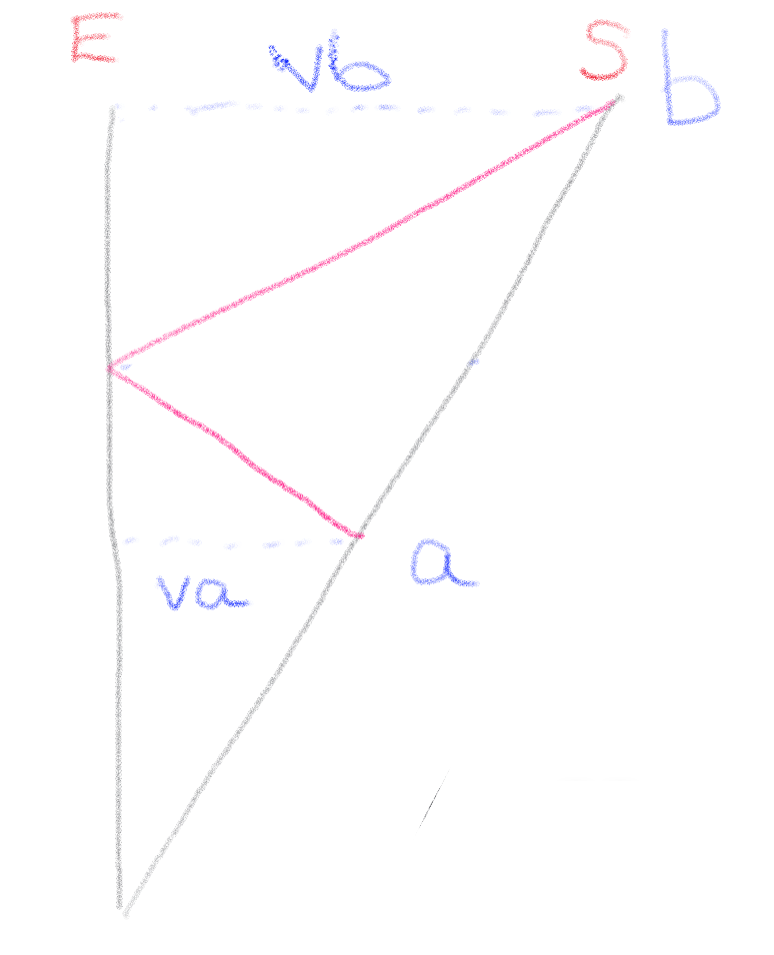
\includegraphics[width=5cm]{sketch2}

% Use radar (or sonar) Relative velocity (as a fraction of c) does not depend on clock
% What B "sees", what A "sees". Doppler effect.
% Applying Doppler effect, now what happens if we assume slow clock?

% Symmetry, even though we know that there is an asymmetry. This is at the root of the twin paradox. There is a fundamental symmetry

% End note: not assuming that speed of light is the same for all observers.

% Would like to jump in right now and apply to twin paradox.
% Whole setup.
% Twin paradox a bit more difficult because we don't know relative velocity for most of the trip. Use of radar does not work.

% Clock paradox (three clocks paradox). Radar stations. Convenient. Overlap problem (but we don't mind for now). Can now work out relative velocity and dedice timing of other clock by application.

% Out - short. In - long. ??? HOw does this resolve PROBLEM.


\section*{Moving clocks run slow world}
% Lorentz transformation
% Not relativity
% Rods not clocks
\section*{extras}

% Hafele experiment
% http://www.personal.psu.edu/rq9/HOW/Atomic_Clocks_Predictions.pdf

\end{document}
